\documentclass{article}

\usepackage{amsmath}
\usepackage{amssymb}
\usepackage{authblk}
\usepackage{color}
\usepackage{graphicx}
\usepackage{lineno}
\usepackage{natbib}
\usepackage{setspace}
\usepackage{url}

\linenumbers

\title{Supplement to Detection of slow slip events using wavelet analysis of GNSS recordings}
\author[1]{Ariane Ducellier}
\author[2]{Kenneth C. Creager}
\author[2]{David A. Schmidt}
\affil[1]{Corresponding author. University of Washington, Department of Earth and Space Sciences, Box 351310, 4000 15th Avenue NE Seattle, WA 98195-1310}
\affil[2]{University of Washington, Department of Earth and Space Sciences}
\date{}

\renewcommand{\thefigure}{S\arabic{figure}}
\renewcommand{\thetable}{S\arabic{table}}

\begin{document}

\maketitle

\begin{figure}
\noindent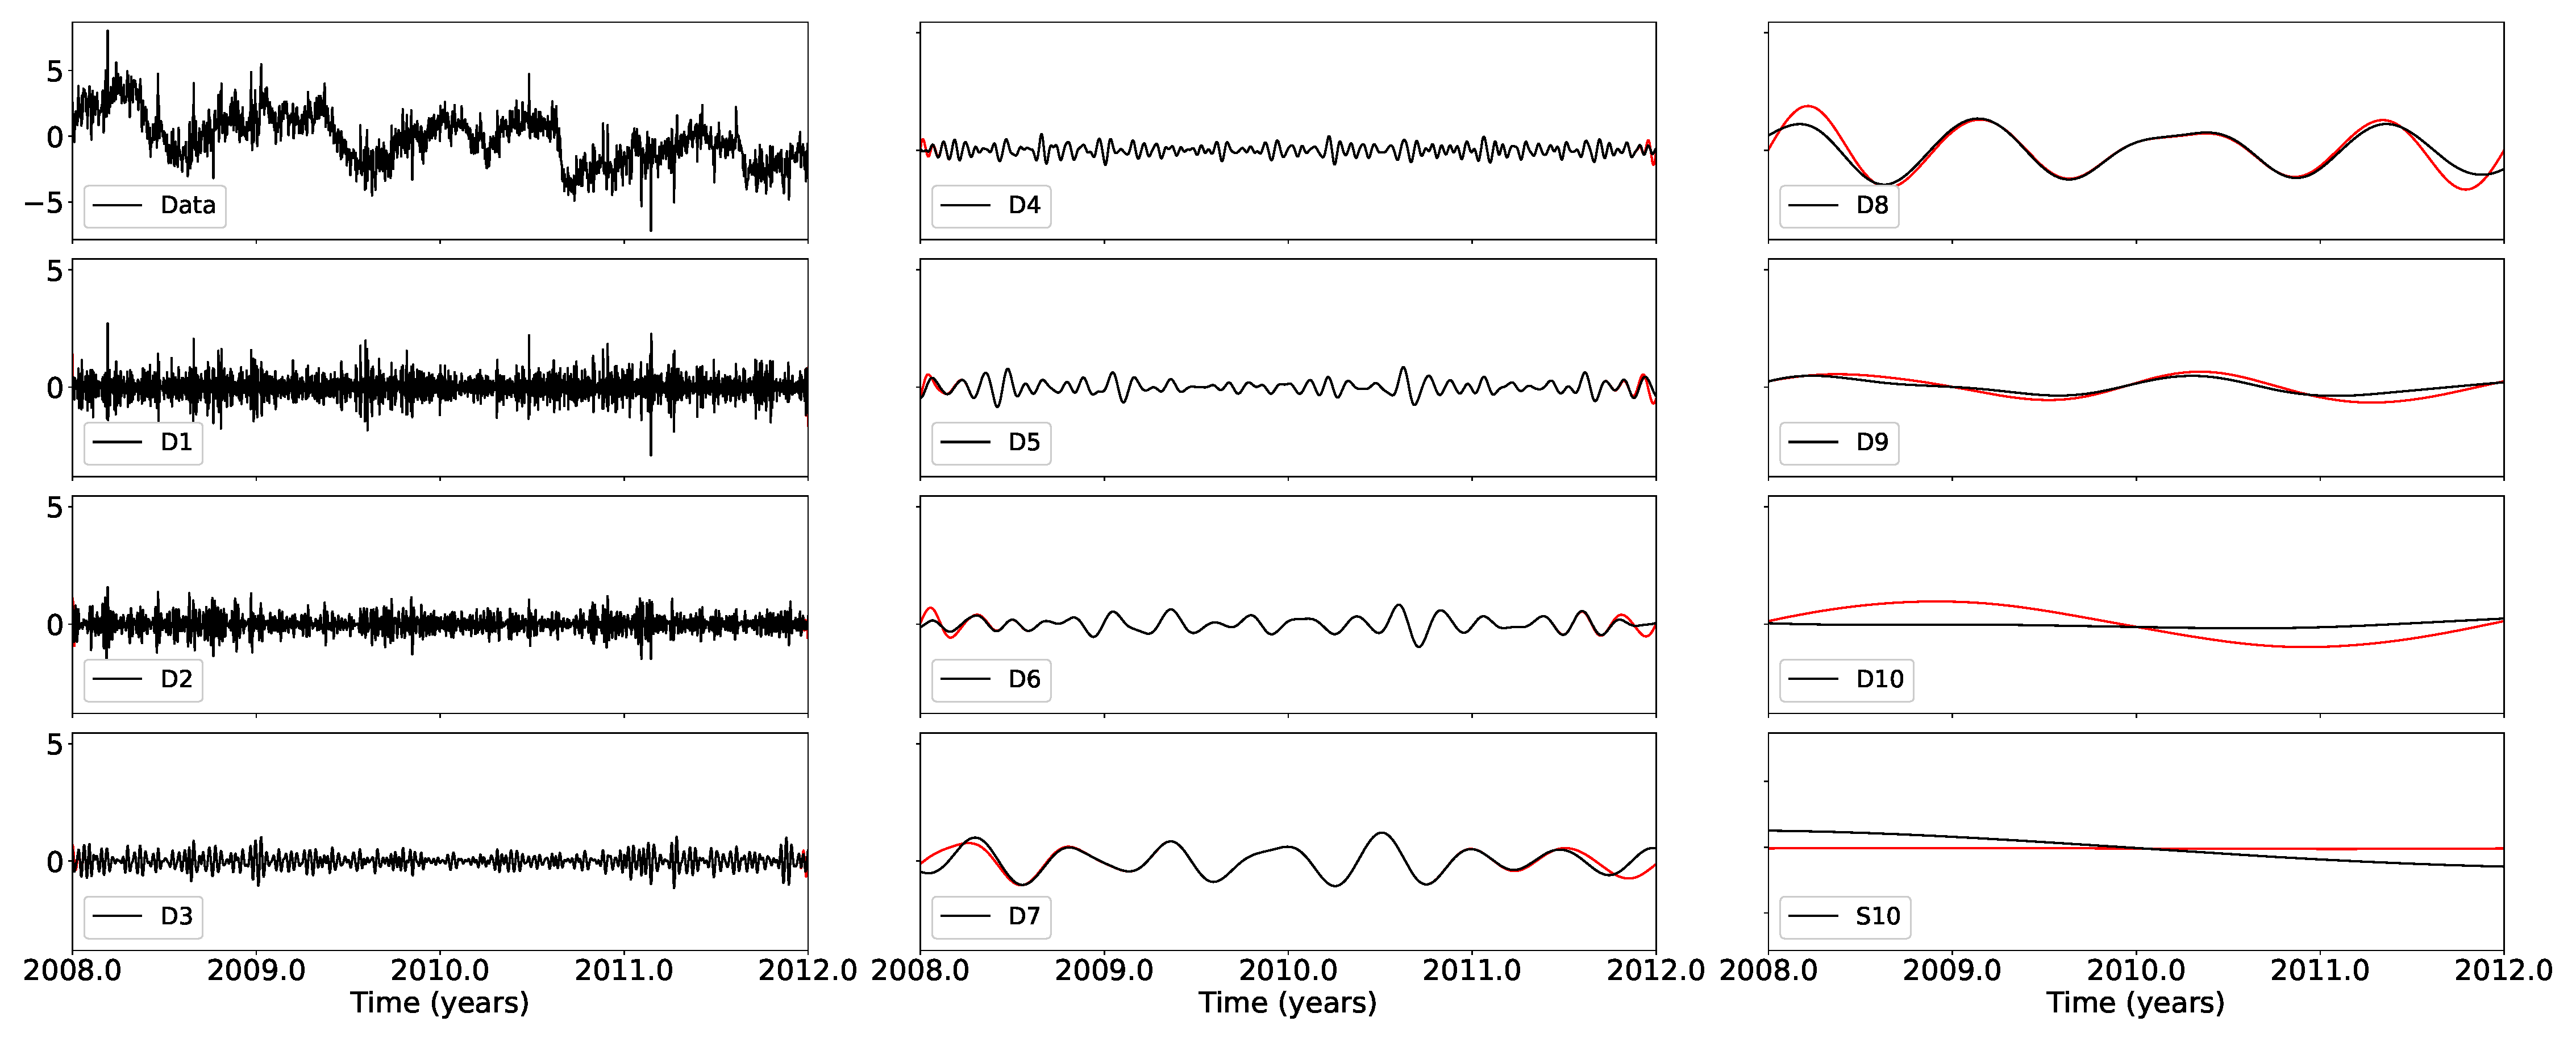
\includegraphics[width=\textwidth, trim={0cm 0cm 0cm 0cm},clip]{figures/boundaries.eps}
\caption{Top left: East-west displacement recorded at GPS station PGC5. Top to bottom and left to right: Wavelet details and smooth computed using only the data from 2008 to 2012 (red) and using the entire time series from 2000 to 2021 (black).}
\label{pngfiguresample}
\end{figure}

\begin{figure}
\noindent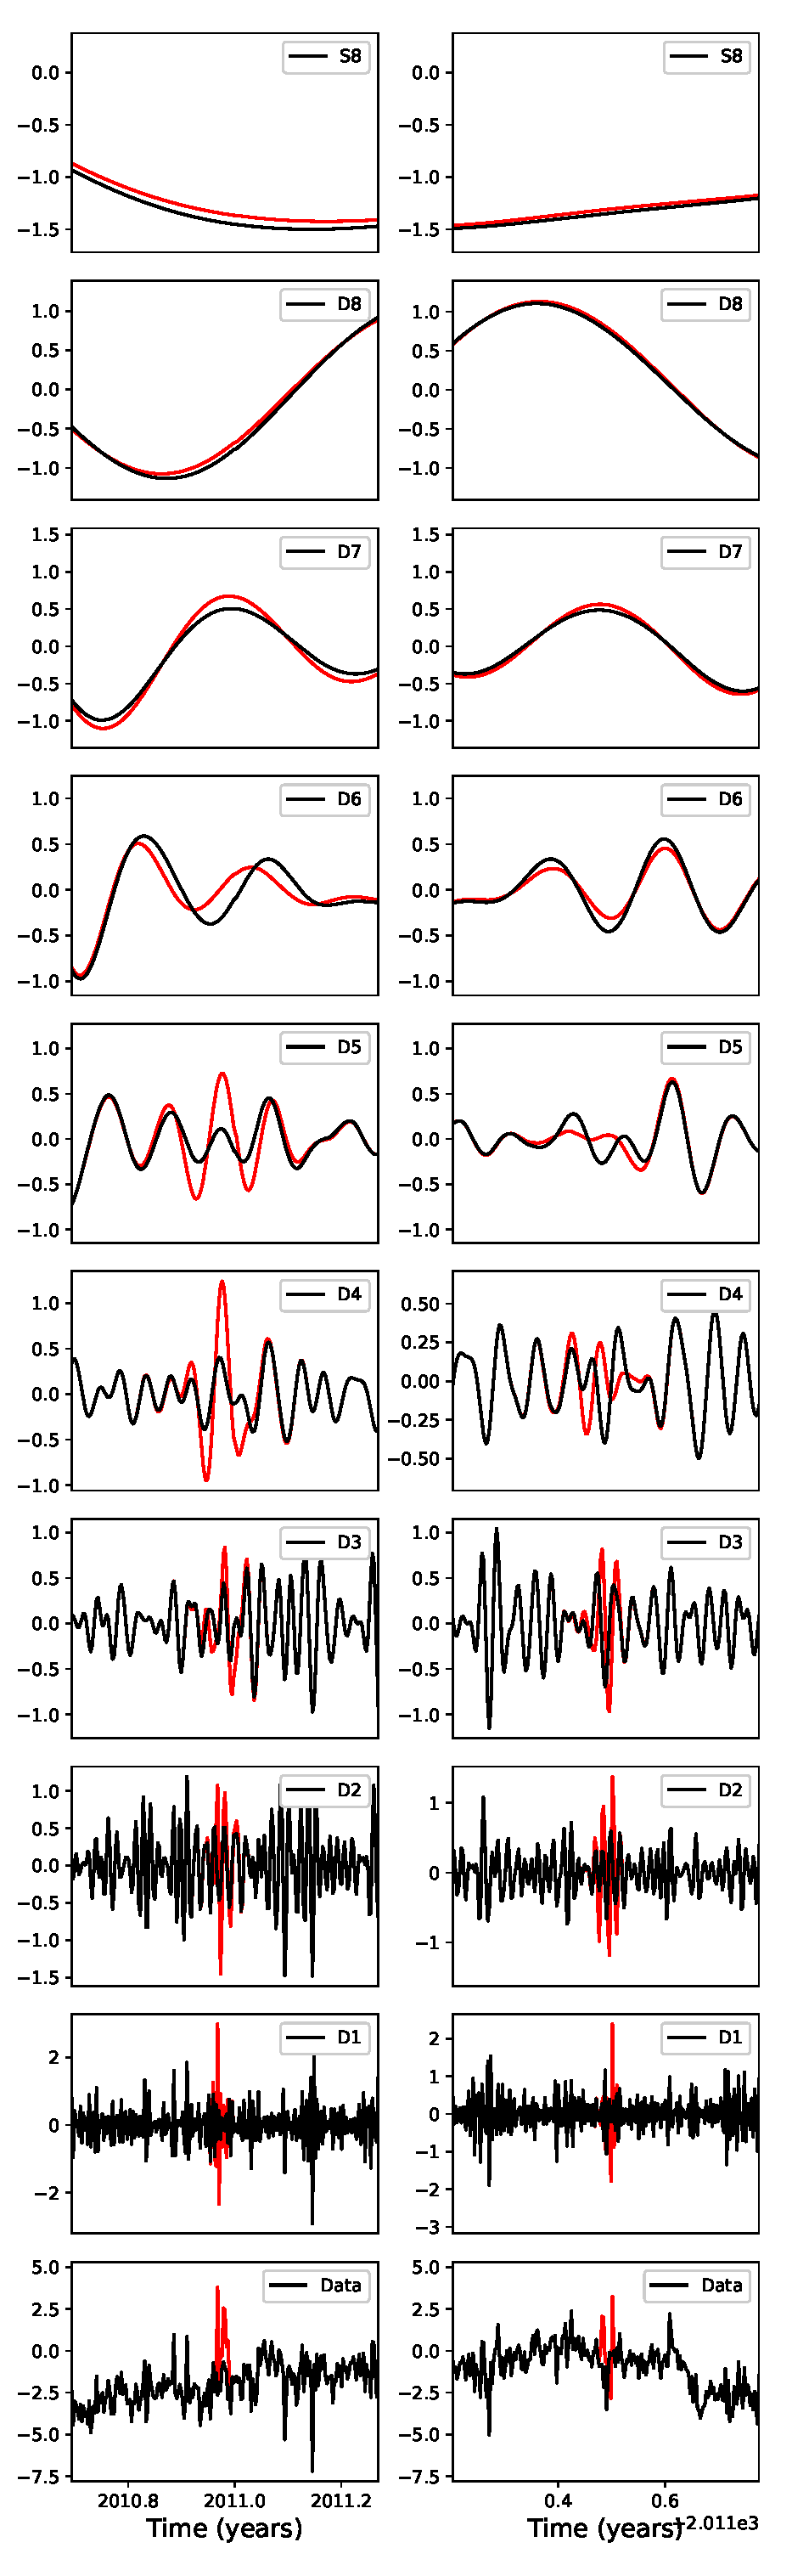
\includegraphics[width=\textwidth, trim={0cm 0cm 0cm 0cm},clip]{figures/DS_10.eps}
\caption{Original data from GPS station PGC5 (black) and same data where displacement values have been artificially removed at two different times (2010.97 for the first four rows and 2011.48 for the last four rows) and replaced by the sum of a straight line and a Gaussian noise component (red). The corresponding ten details and smooths of the wavelet composition are shown in increasing levels for the original data (black) and for the data with displacement values removed and replaced by linear interpolation plus Gaussian noise (red).}
\label{pngfiguresample}
\end{figure}

\begin{figure}
\noindent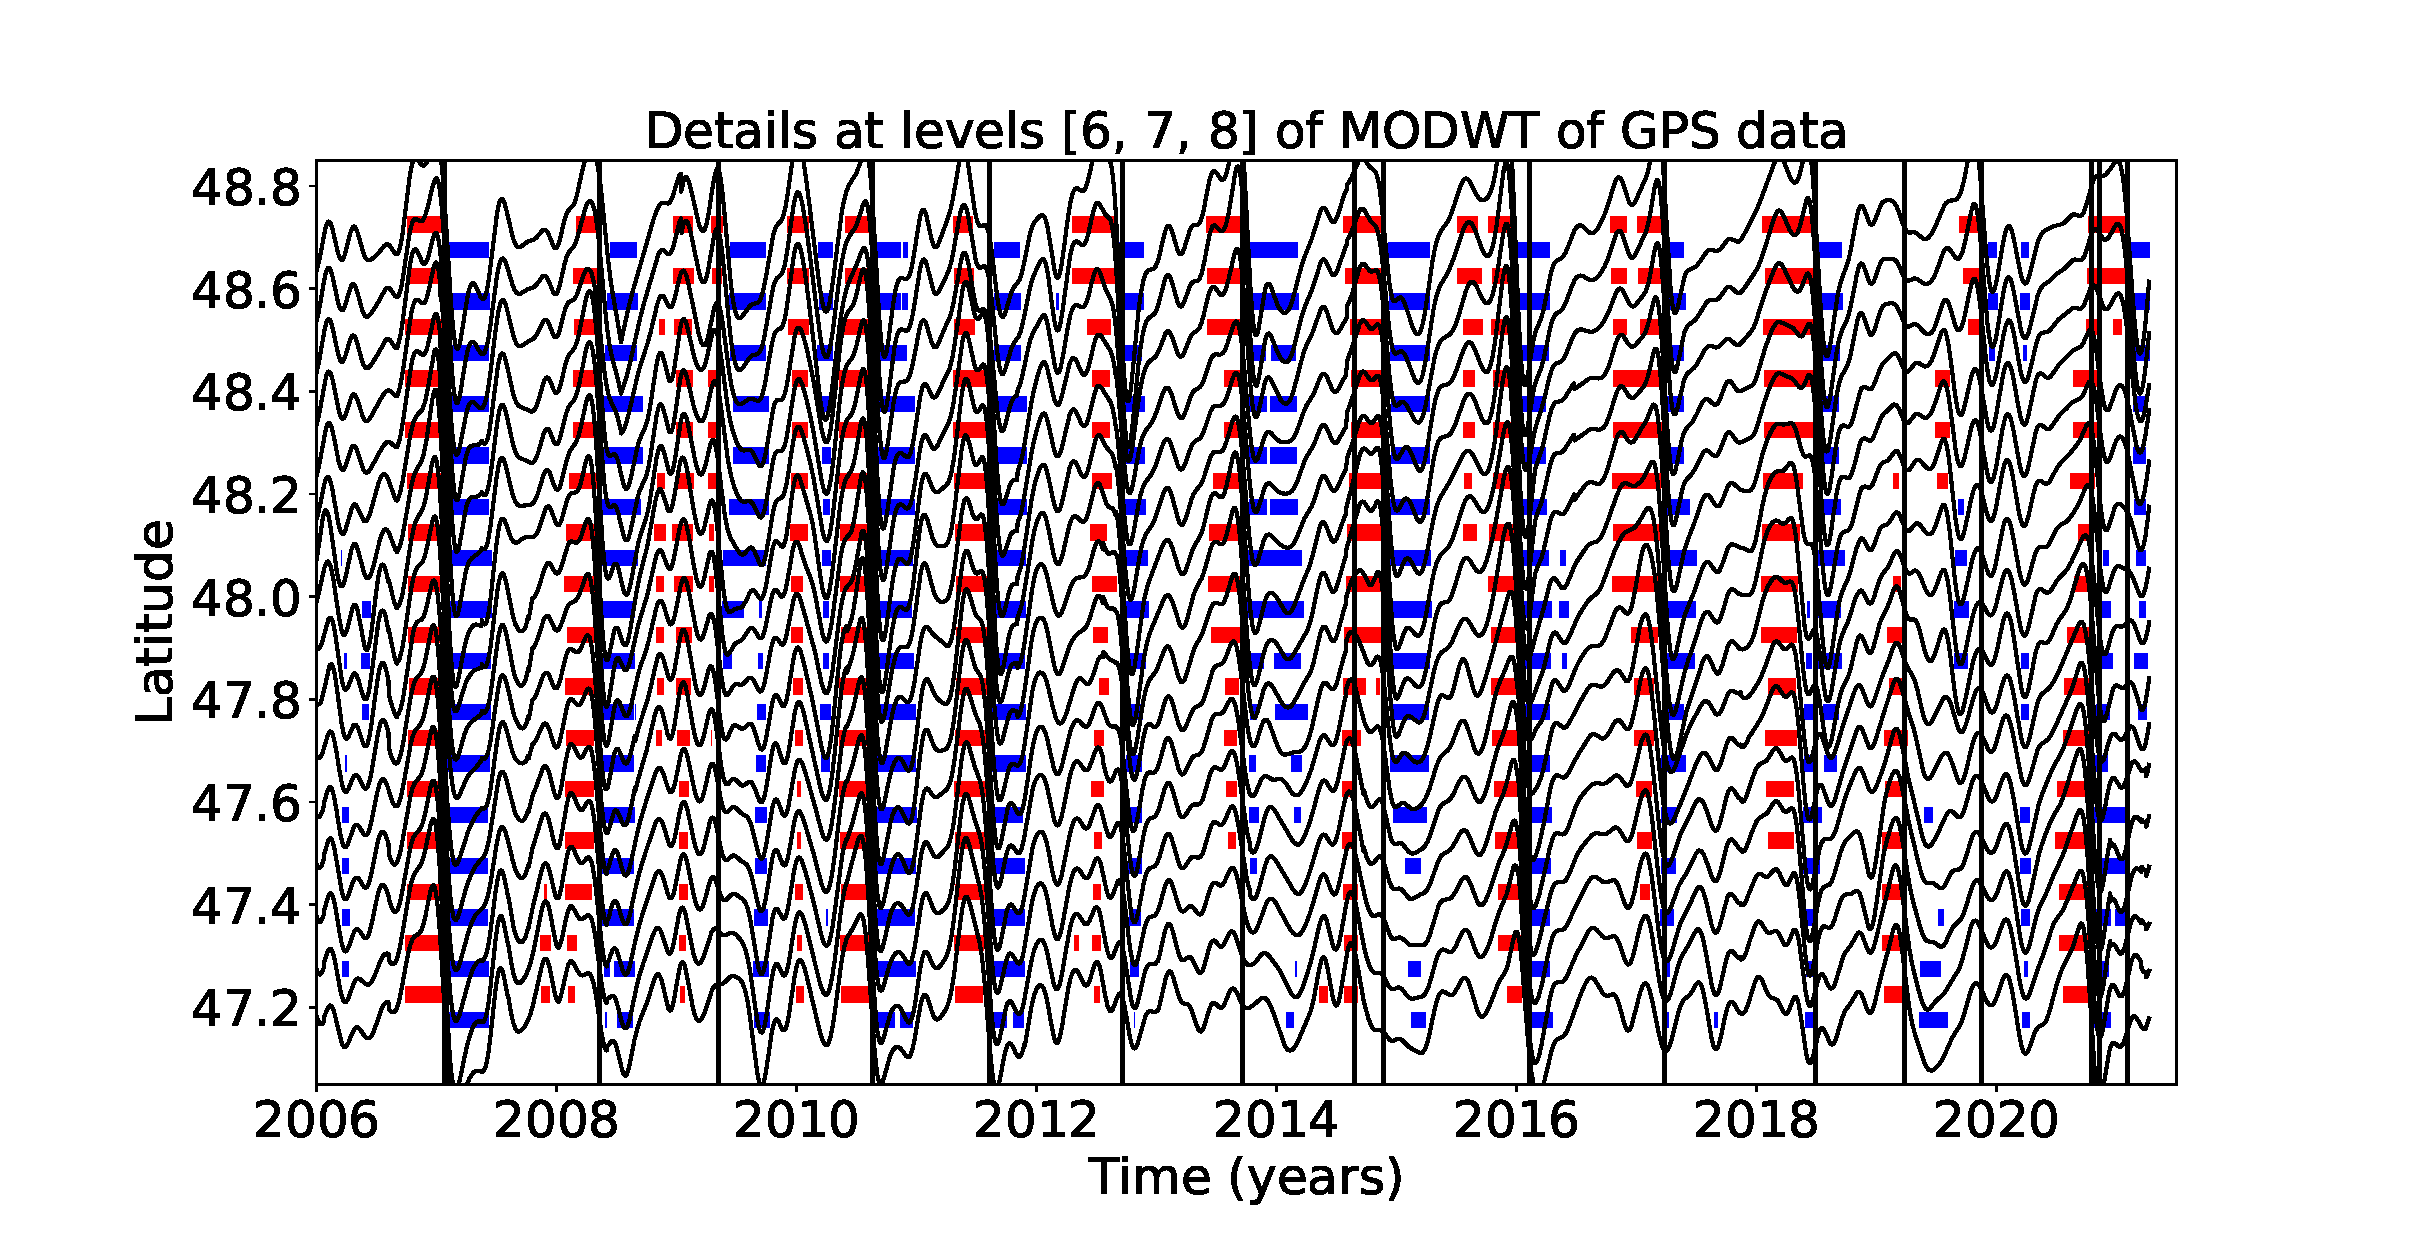
\includegraphics[width=\textwidth, trim={0cm 0cm 0cm 0cm},clip]{figures/GPS_mode_details_6-7-8.eps}
\caption{Same as top panel of Figure 9 from the main text, but using the GNSS time series where common modes have been removed before applying the wavelet transform.}
\label{pngfiguresample}
\end{figure}

\begin{figure}
\noindent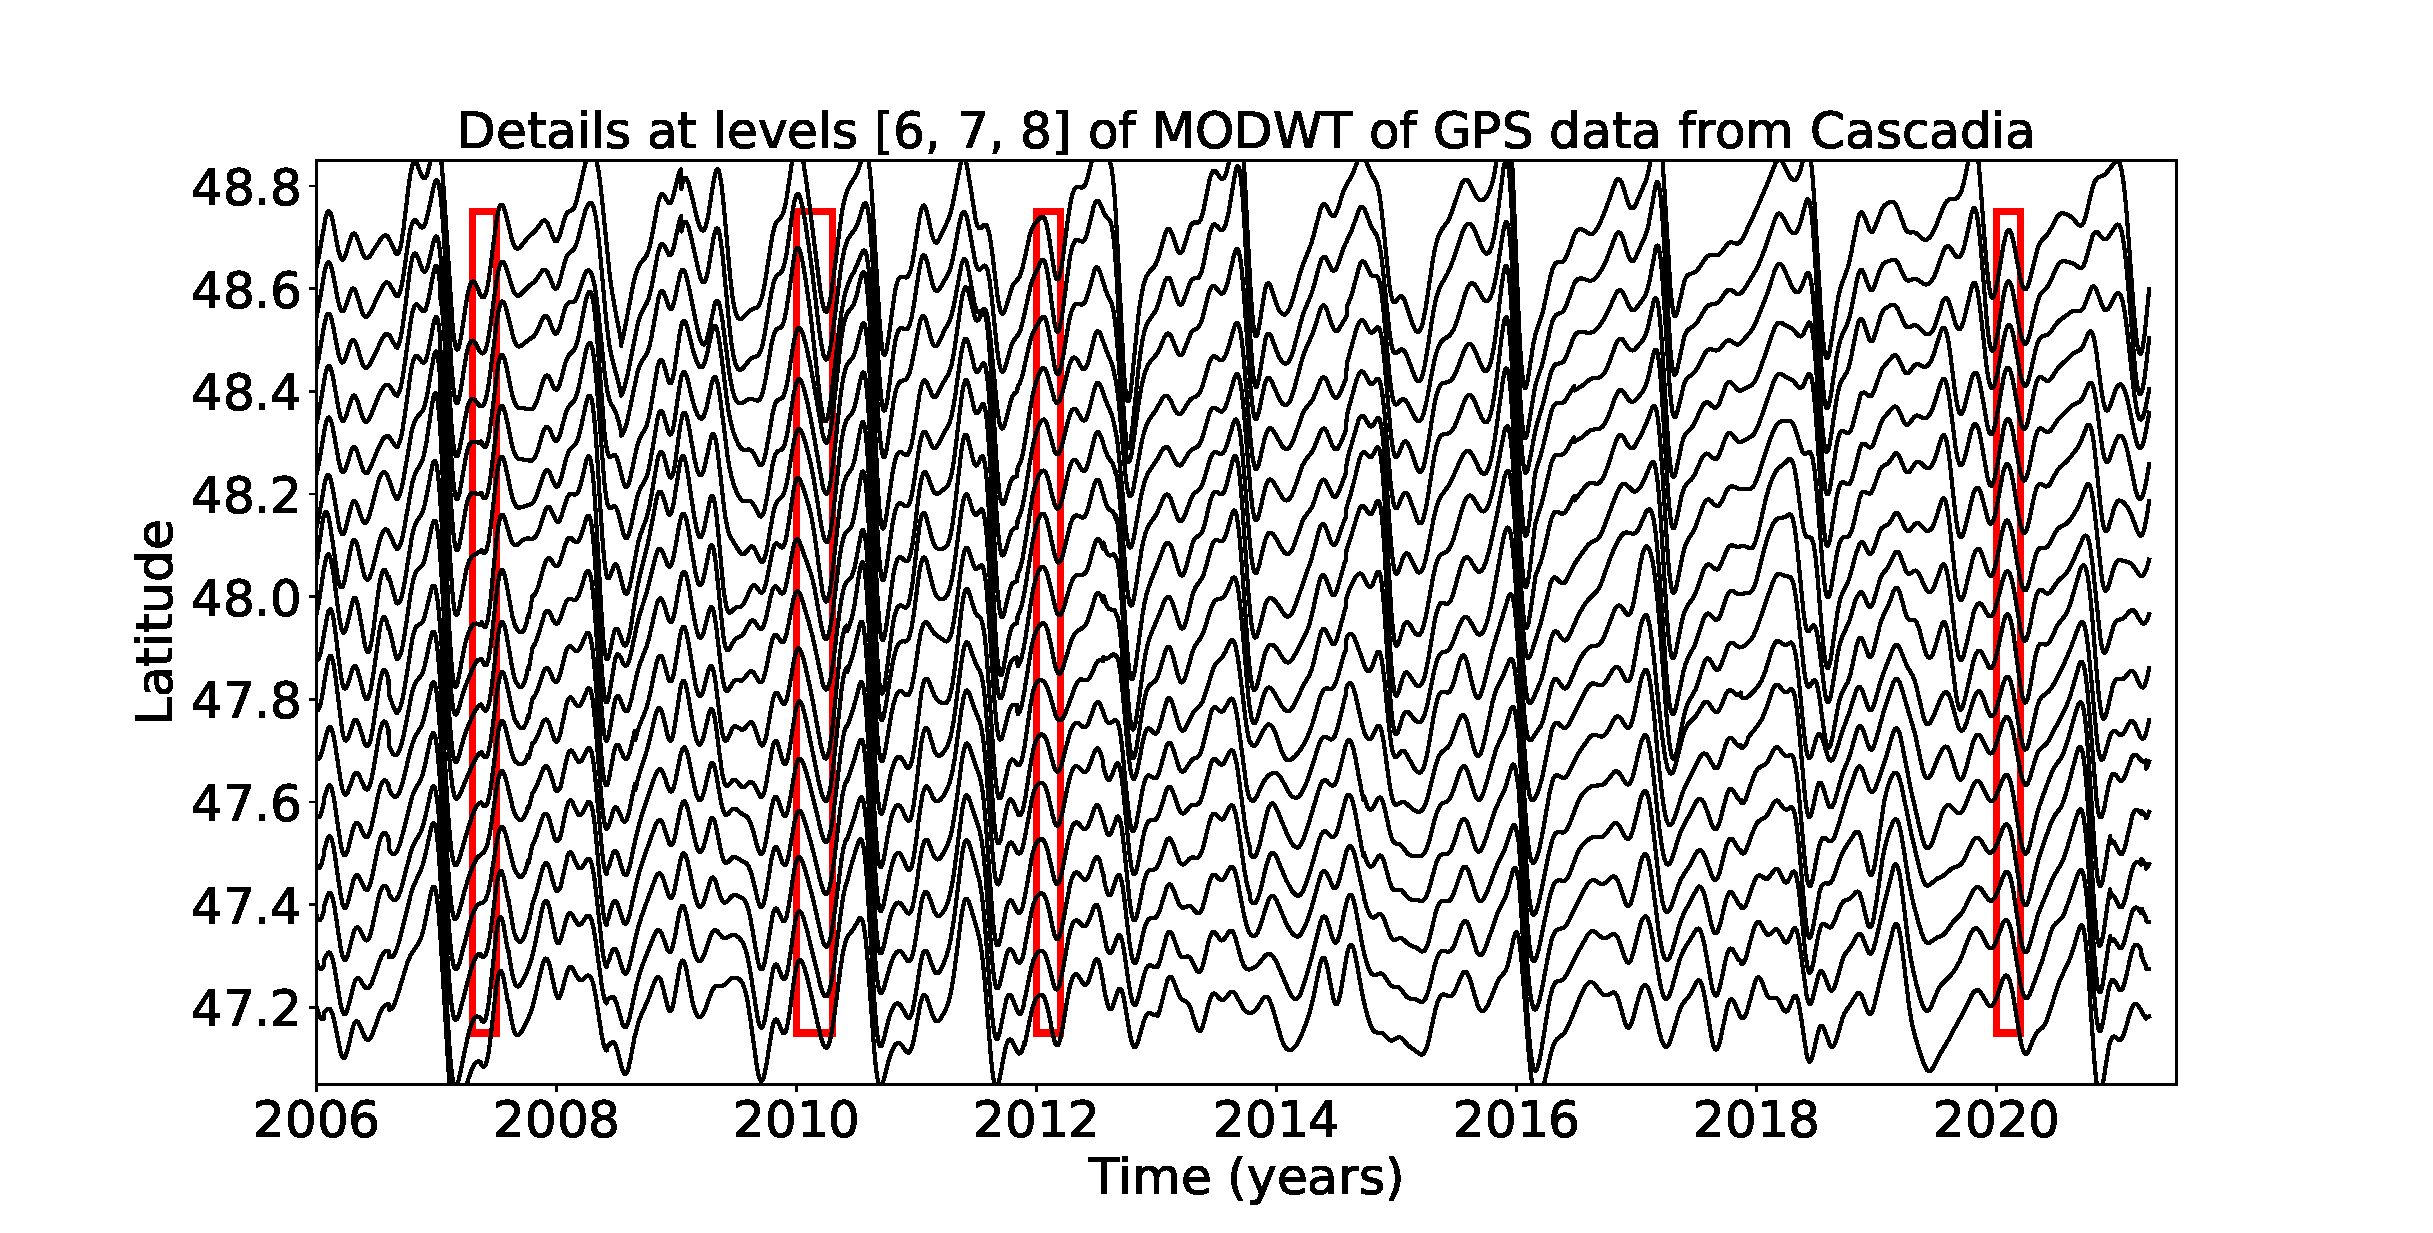
\includegraphics[width=\textwidth, trim={0cm 0cm 0cm 0cm},clip]{figures/GPS_longer_details_6-7-8_events.eps}
\caption{Same as top panel of Figure 9 from the main text. We highlight by four red rectangles the four possible small transients discussed in the text.}
\label{pngfiguresample}
\end{figure}

\end{document}
